\documentclass[12pt,letterpaper]{article}

%==================================================================================
% Template for the 13th International Association of Fire Safety Science (2019).  
%==================================================================================

% This template is based on the layout requirements of the Fire Safety Journal.  When submitting, please do include the *.tex and output (typeset) *.pdf files, figure files (photographs, diagrams, etc.), and any other ancillary files required to typeset your article.  The journal must be able to typeset your article with what you've provided.

% As with any programming language, there are multiple ways of executing any given task (e.g., figures, tables, maths, etc.).  The syntax in this template should be considered suggestions and not directives.  Please feel free to use your own favorite syntax, especially if it's more elegant than what is found below!  That said, the spacing and font parameters have been selected to conform to the appearance dictated by the journal (i.e. like MS Word).  Make sure your final typeset document has the correct formatting or it will be rejected.

% Required Packages ===============================================================
\usepackage{amsmath} % The usual maths package
\usepackage{amsfonts}  % The usual maths package
\usepackage{amssymb}  % The usual maths package
\usepackage[final]{graphicx} %Required for figures.
\usepackage{footnote}
\usepackage{footmisc}
\usepackage{caption} % Needed to modify default figure captions
\usepackage{latexsym}
\usepackage{lineno} % Enables line numbers
\usepackage{parskip} % Makes a space between paragraphs like MS word
\usepackage{fullpage} % Overrides article margins
\usepackage{titlesec} % Enables modification of section labels
\usepackage[numbers,sort&compress]{natbib}
%\usepackage[numbib]{tocbibind} %Make References a numbered section
\usepackage{siunitx} % Formats the units and values
\usepackage{times}
\usepackage{chemformula}


%\usepackage{subcaption} % Enables multiple images in one figure environment
%\usepackage{xcolor} % For various font colors in figures
%===================================================================================

% The next two lines modify the font and font size of the section and subsection labels
\titleformat{\section}{\normalfont\bfseries}{\thesection}{0.2em.}{}
\titleformat{\subsection}{\normalfont\bfseries}{\thesubsection}{0.2em}{}

% This will change the figure captions from the default "Figure 1:" to "Fig. 1."
\captionsetup[figure]{labelformat={default},labelsep=period,name={Fig.}}

\linenumbers % Include line numbers throughout document

\newcommand\numberthis{\addtocounter{equation}{1}\tag{\theequation}}

\begin{document} %====================================================================
\begin{flushleft} % Suppress the default full justification of text

% Title of your article
\textbf{A study on local conditions conducive to deflagration in a scaled compartment}
\vspace{3mm}\\
%
% Author(s)
Marcos Vanella$^\text{a*}$, Chandan Paul$^\text{a,b}$, Thomas Cleary$^\text{a}$, Ryan Falkenstein-Smith$^\text{a}$
\vspace{3mm}\\	

% Affiliation "b"
$^\text{a}$National Institute of Standards and Technology, 100 Bureau Drive, Gaithersburg, USA  \\
$^\text{b}$The George Washington University, 800 22nd Street, NW, Washington DC, USA  \\
\vspace{3mm}

$^*$Corresponding author : marcos.vanella@nist.gov

% Highlights/keywords ===================================================
%\textbf{Highlights:}	
%\begin{itemize}
%	\itemsep-4pt % Override default vertical spacing among list items
%	\item A series of backdraft experiments were conducted in a reduced-scale enclosure
%	\item Different methane and propane fire configurations were implemented to vary the gas mixture distribution and internal density
%	\item The gas mixture density within the enclosure was observed to impact the mixing dynamics of the gravity current as it entered the compartment
%	\item Ignition was achieved for rich gas mixtures surrounding a charged spark ignitor
%	\item \textcolor{black}{A relationship between the total heat release of the resulting backdraft and the initial mass fraction of fuel residing within the enclosure was observed} for experiments utilizing propane
%\end{itemize}
%\vspace{3mm}

% Abstract ==============================================================	
\textbf{Abstract:}

\vspace{3mm}


\textbf{Keywords:}
Enclosure Fire; Gaseous Fuels; Backdraft; Experiments; Numerical Simulation

\section{Introduction} \addvspace{10pt}
\label{sec:introduction}

Backdraft - what it is, lit review. Local conditions conducive to flame propagation within the compartment. Mixing, critical fuel mass.

- Simulations, lit review, 2-3 equation kinetics for combustion, arrhenius vs fast chemistry.

- Purpose of this work - study flame propagation potential comparing to experiments done at NIST. We are talking about deflagration initiation with spherical flame with diameter up to several centimeters. In this scenario fully mixed fuel and oxygen can be assumed. Other than that, the flame will move into regions where combustion can be mixing controlled (into the gravity current) and pressure generation affects the dynamics of the compartment ejecting fuel, oxygen and products through the door. What affects the flame viability? Do profiles of temperature, fuel, initial Oxygen with height have an effect? 

\section{Experimental Setup} \addvspace{10pt}
\label{sec:expsetup}

\subsection{Definition of Initial conditions} \addvspace{10pt}
\label{sec:initcond}


\subsection{Numerical Model} \addvspace{10pt}
\label{sec:nummodel}

In order to simulate the gravity current incursion and record composition and temperature values with time in designated positions within the compartment we defined a model and used FDS (FDS-6.9.1, commit \textit{7e7cd3b} source code from May $21^{st}$, 2024) in large eddy simulation (LES) mode. The compartment and burner geometries were specified together with devices to sample composition and temperature in and around the ignitor locations used in experiments. Adiabatic conditions were prescribed in compartment and burner surfaces, neglecting heat transfer on this fast transient problem. Different initial conditions as described in the previous section were used with the compartment in open door configuration to simulate the cold air flow into it and gravity current development. The computational domain was optimized to record the flow of air and species within the compartment and across the compartment door as seen in Figure~\ref{}a. 


Three grid resolutions were used to evaluate grid sensitivity. These employed cell sizes $\Delta x=0.25$ cm, $\Delta x=0.5$ cm and $\Delta x=1$ cm. For $\Delta x=1$ cm, the domain was split in 304 meshes with $(28\times32\times26)$ cells. For the cases $\Delta x=0.5$ cm and $\Delta x=0.25$ cm, 608 $(56\times32\times52)$ and 2432 $(56\times64\times52)$ meshes were used respectively. All cases were run for 8 s of simulation time in the Frontera supercomputer~\cite{frontera}, an amount of time deemed sufficient to effectively deplete the fuel in compartment. It took from 30 minutes to 16 hours of wall time to complete these calculations. Parallelization was based on using one mesh per MPI rank, and one MPI rank per CPU core. Therefore, up to 2432 cores were used in the machine. A slice of oxygen volume fraction depicting the gravity current after door opening for the finest grid resolution is shown in Figure~\ref{}b.   

% Figure: a) 304 mesh setup b) Oxygen volume fraction at 1.X sec after door opening:


Global measures of grid sensitivity chosen are total fuel mass in the compartment $M_{C_3H_8}$ at half the simulation time t=4 s, as well as outbound fuel mass flow through the door $\dot{M}_{C_3H_8}$ and average gravity current height $H_G$. 
$H_G$ was computed as the distance from the floor where the time averaged normal velocity profile recorded in the door symmetry plane alternated sign (change form inflow to outflow). 
These give a good perspective on the mean composition evolution in the compartment and fluid mechanics resolution. Values for these quantities and differences respect to the finest  $\Delta x=0.25$ grid solution are provided in Table~\ref{tab:errgrid} for initial composition and temperature conditions gathered from the FFT=300s experiments. It is noted that all grid resolutions agree on these quantities within 5\%.

% Table of global sensitivity measures and error:
\begin{table}[h!]
\caption{Global measures of convergence for FFT=300 s, propane fuel case.}
\label{tab:errgrid}
\centering
\footnotesize
\begin{tabular}{l c c c c c c}
\hline
Grid Size & $M_{C_3H_8}$ (gr)	& $\Delta M_{C_3H_8}$ (\%) & $\dot{M}_{C_3H_8}$ (gr/s) & $\Delta \dot{M}_{C_3H_8}$ (\%) & $H_G$ (cm) & $\Delta H_G$ (\%)\\
\hline
$\Delta x=1$    cm & 62.0 & -2.2 & 6.17 & 4.53  & 47.0 & 3.1 \\
$\Delta x=0.5$  cm & 63.2 & -0.3 & 6.02 & 2.07  & 47.1 & 3.3 \\
$\Delta x=0.25$ cm & 63.5 &      & 5.89 &       & 45.6 &  \\
% Methane & 25.0~$\pm$~1.0~kW 	& 360,~390,~450\\
% 	& 37.5~$\pm$~1.0~kW 	& 225,~285      \\
% %[0.075cm]
% Propane & 16.7~$\pm$~1.0~kW		& 255,~270,~315	\\
% 	& 25.0~$\pm$~1.0~kW 	& 210,~285		 \\
\hline
\end{tabular}
\end{table}



Two ignitor locations were defined as low-ignitor (LI) and mid-ignitor (MI). The first was defined in the symmetry plane of the compartment at about 1 m from the door and 25 cm from the floor. The latter was defined also at 1 m from the door but at mid height of the compartment. Star clusters of 7 sampling devices were defined to note mixture composition and temperature at each ignitor location, and at 2 cm in every coordinate direction around it as shown in Figure~\ref{}a.

In Figures~\ref{fig:CompSetup}a,~\ref{fig:CompSetup}b local fuel and oxygen variations with time are shown at the LI, MI locations for FFT=300s and different grid resolutions. We noted on this case and others, for both LI, MI locations there was no significant difference in gas composition and temperature among the different mesh resolutions. Therefore, the analysis presented on this work is based on 1 cm grid resolution calculations.

% Figure: a) 7 point stencil of devices aroun LI ignitor location, b) LI location 300s FFT LI,MI fuel and oxygen volume fraction with time.
\begin{figure}[tb]
    \centering
    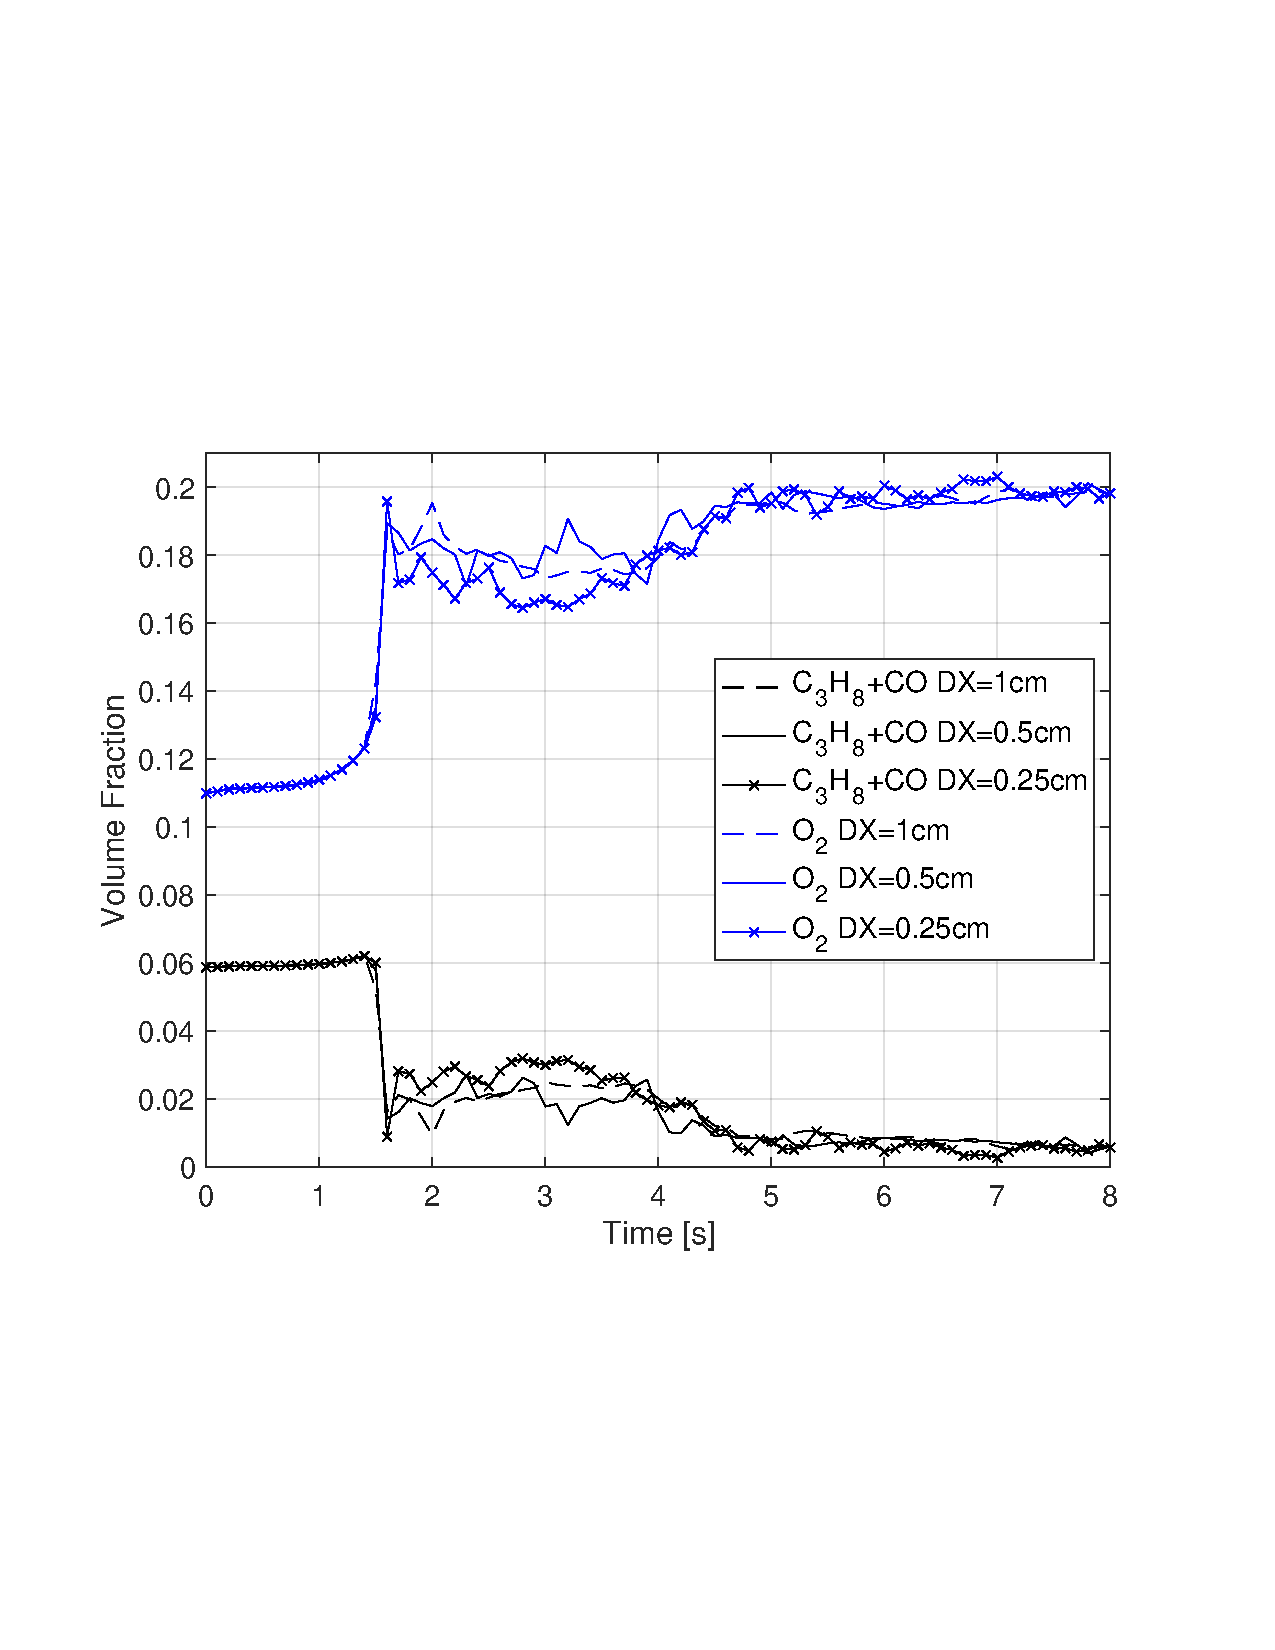
\includegraphics[trim = 14.5mm 65mm 17mm 70mm, clip,width=0.505\textwidth]{AOSFST_Paper/Figures/Low_Ignitor_Comp_Tvar_300s.pdf}
    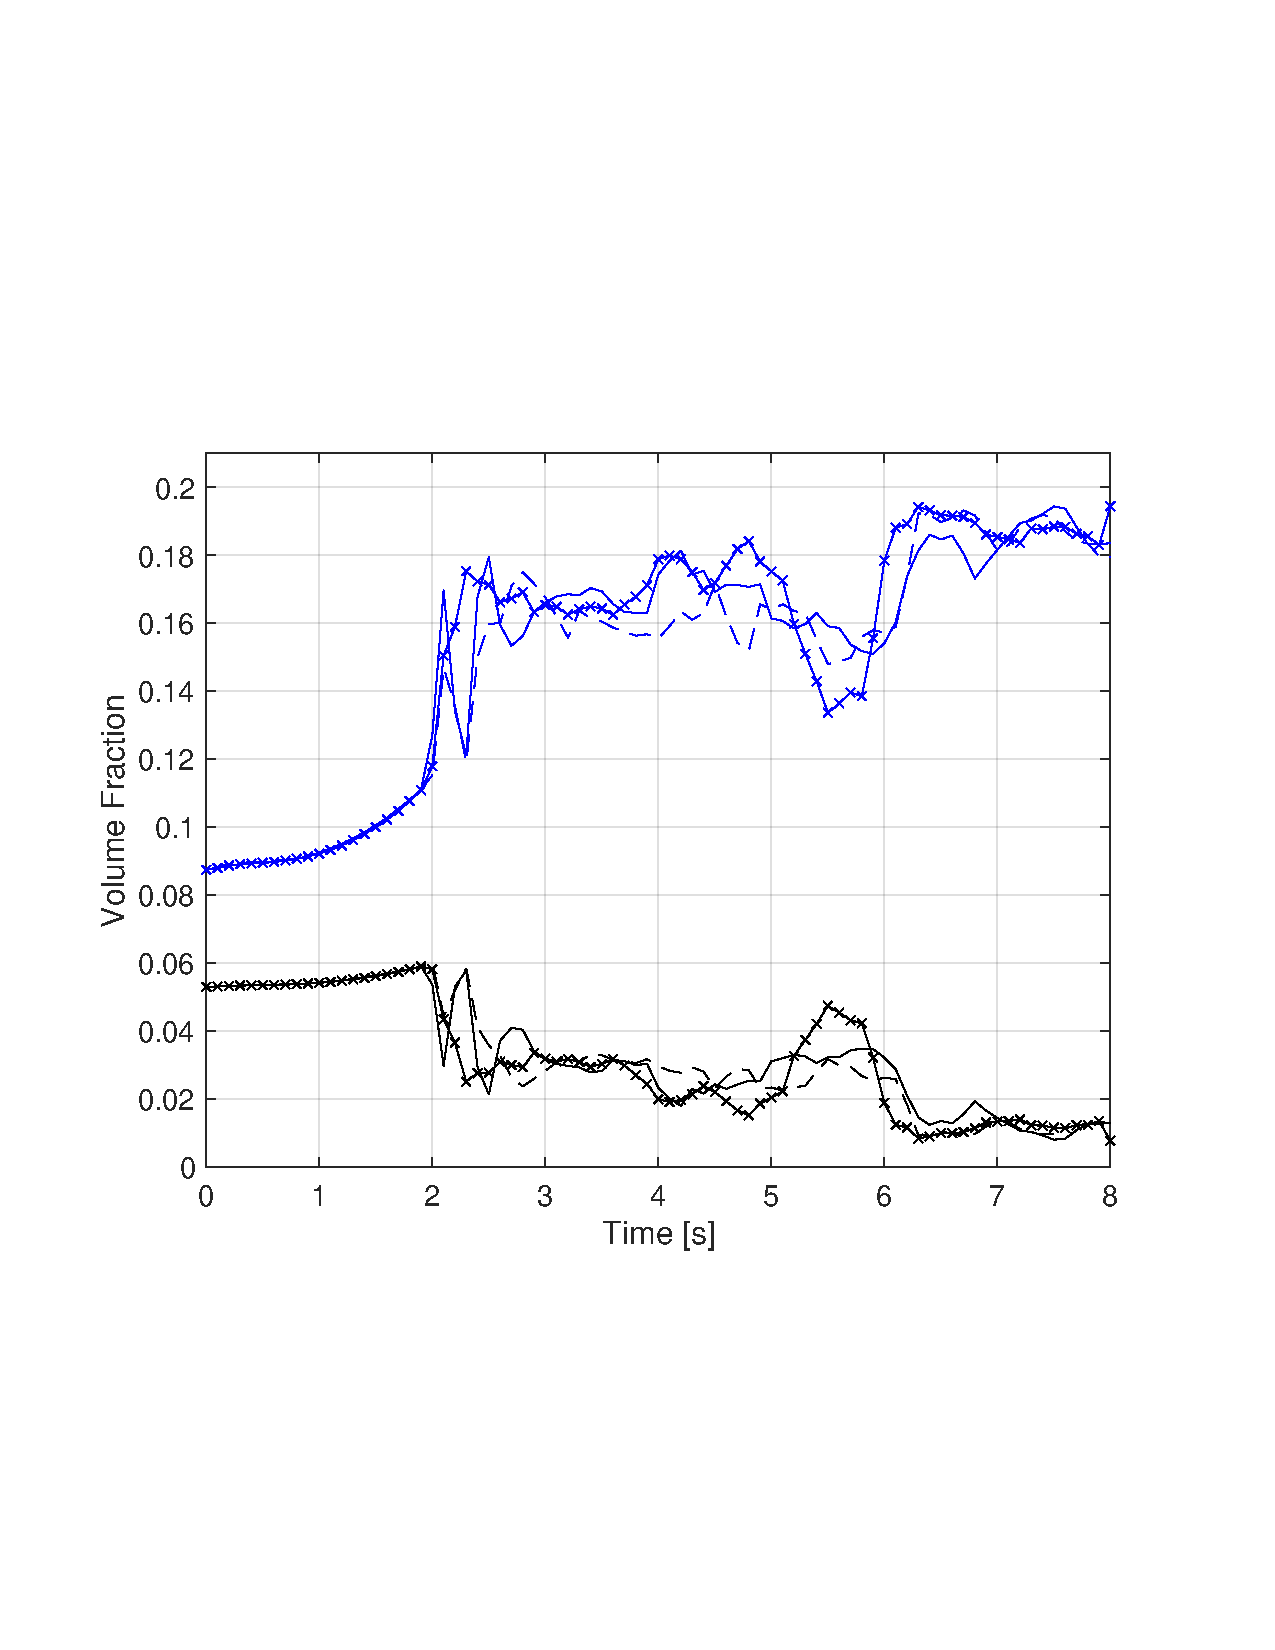
\includegraphics[trim = 22mm 65mm 17mm 70mm, clip,width=0.485\textwidth]{AOSFST_Paper/Figures/Mid_Ignitor_Comp_Tvar_300s.pdf}
    \makebox[0.50\textwidth]{(a)}
    \makebox[0.48\textwidth]{(b)} \\
    \caption{Local mixture composition as a function of time for different grid resolutions: (a) Low-ignitor (LI), (b) Mid-ignitor (MI). }
    \label{fig:CompSetup}
\end{figure}



\textbf{- Defining conditions for flame propagation - Flammability diag/Cantera methodology.}






\subsection{Results} \addvspace{10pt}
\label{sec:results}

\subsection{Effect of compartment fuel loading}
\label{sec:resfuel}


\subsection{Effect of compartment oxygen content}
\label{sec:resfuel}


\section{Conclusions}



 

%\section*{References}
\bibliographystyle{elsarticle-num}
\bibliography{References}
\end{flushleft}
\end{document}